
\tightsection{Implementation and Production Deployment}
\label{sec:eval}

\begin{figure*}[t!]
\centering
\subfigure[Daily improvement (both metrics)]
{
  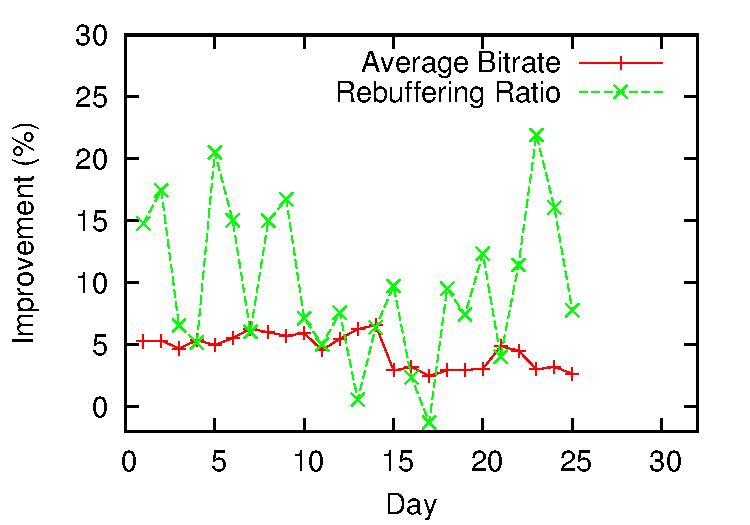
\includegraphics[width=0.3\textwidth] {figures/eval-perfimp.pdf}
  \label{subfig:buffering-and-bitrate}
}
\subfigure[Buffering ratio (\%): GO vs. per-CDN]
{
	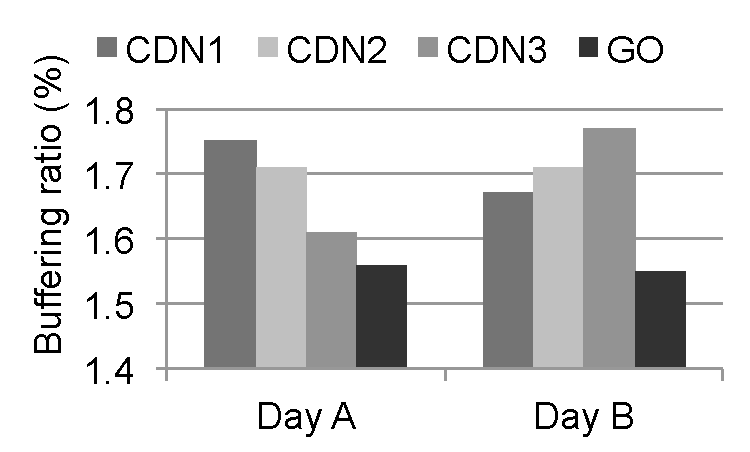
\includegraphics[width=0.3\textwidth]{figures/ab-testing-figures/bufferingratio-new.pdf}
	\label{subfig:eval-case-study:bufferingratio}
}
\subfigure[Avg. bitrate (Kbps): GO vs. per-CDN]
{
	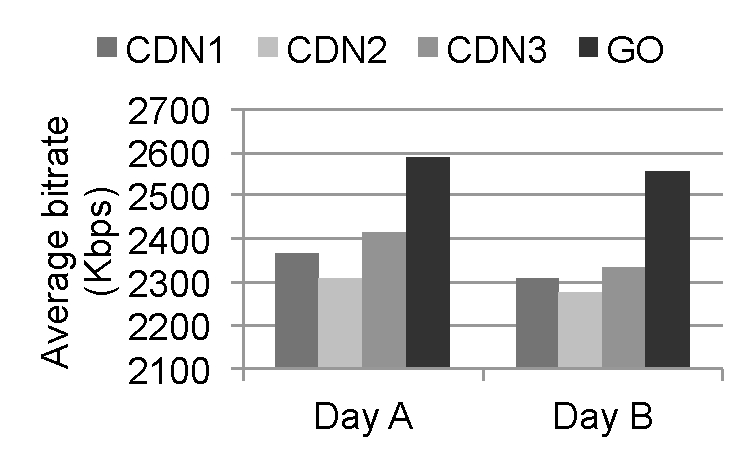
\includegraphics[width=0.3\textwidth]{figures/ab-testing-figures/averagebitrate-new.pdf}
	\label{subfig:eval-case-study:averagebitrate}
}
\tightcaption{Performance Metrics and Improvement from GO}
\label{fig:perf-impr}
\end{figure*}



\tightsubsection{Implementation}
\label{sec:impl}

While there are many details in the building of the GO system, we focus our discussion on two main components: pre-computation and on-line decision making. In order to achieve fast on-line decision making, the GO system has a pre-computation module that (a) computes and updates an AC partition table periodically, and (b) broadcasts the computed table to a set of distributed decision servers that will use the table to make on-line decision making upon requests of clients. 

AC partition table generation is essentially the process of aggregating quality samples into partitions of different ACs and then computing summary statistics for each partition (e.g., mean and standard error of mean).
Our implementation uses Spark~\cite{spark} as the underlying compute framework and is implemented in a single map-reduce stage. 
Quality samples are loaded in parallel from an HDFS source~\cite{hadoop} and distributed amongst the cluster in form of Resilient Distributed Datasets (RDD)~\cite{zaharia2012resilient}. 
%Each node then maps its share of quality samples to a set of preliminary buckets. Common buckets are then shuffled across the cluster and the results are aggregated and collected onto a master machine. 
Currently it takes GO system 12 seconds to process 500K partitions on a 4-node cluster with a total of 64 cores and 512G memory. 
All steps involved in creating the table are horizontally scalable.
We did not spend time to tune the performance of the pre-computation module as it satisfies the requirement of our current deployment where we we re-compute the table between 30 seconds and 1 minute.


The resulting table is broadcasted to a set of of decision makers (DMs) closer to video clients in multiple POPs by way of a distributed messaging system~\cite{kreps2011kafka}. Each entry of the AC partition table is about 100 Bytes uncompressed. For a table of 500K entries, the table is about 50MB.  Assuming an update frequency of one minute, the bandwidth required is 0.83Mbps per POP. Again, we did not tune the performance of this portion of the system as the current implementation satisfies the need for the current deployment scenario. 

Once a decision maker has a table, decision making involves multiple lookups of the table and combines the results from the lookups.  Given that there are $N$ ACs for decision evaluation, and $M$ possible decisions, there are $M \times N$ lookups for a decision to be made. The decision making process is horizontally scalable by adding more decision makers. The average response time from current GO system is $0.62 ^{+}_{-} 0.016$ms, which is insignificant compared to RTT in Internet.

In summary, the current implementation of GO is horizontally scalable and can provide low response times for on-line decision making. 

\tightsubsection{Production Deployment}
\label{subsec:eval_setup}


The GO system is currently deployed in multiple premium publishers. However, there are several practical difficulties of evaluating the performance of GO in production deployment environments.  First, most publishers do not want to perform A/B testing when they understand that the performance of some of the streams may not be optimal when they are grouped by the “non-optimized” version of the algorithm. Second, with all publishers, there are usually additional business considerations beyond the goal of optimizing the QoS of the video streams. For example, when using multiple CDNs, a publisher would get a lower price from a particular CDN if it would allocate more than a certain percentage of its total traffic to the CDN.  This “CDN allocation policy” would put additional constraint on the GO optimization algorithm.  Consider a scenario that a publisher has three CDNs $X$, $Y$, and $Z$, and have minimum committed usage percentage on $X$ and $Y$. This would mean that even if CDN $Z$ is the best performing CDN based on the prediction algorithm, beyond certain percentage of traffic, no additional streams would be allocated to it. 

In this section, we are presenting performance results from one publisher who has agreed to allow us to do A/B testing in production with iOS devices (both iPhone and iPad) on their short-form videos (5 minutes).  In this deployment, the publisher utilizes three CDNs with minimum committed percentage usage on each of them and encodes video in 5 bitrate levels (from 700Kbps to 3.5Mbps).The publisher uses the GO system to select the CDN and the nitrate at the start of each session.  The video app is using Apple’s native player for video playback and  HLS protocol as the adaptive 
bitrate switching algorithm to change the bitrate during the video session (without CDN switch). 
 
The results are collected from Jan 1st, 2014 to Jan 25th, 2014 (total of 25 days) with 26.1 million sessions (870K sessions on average per day).
We compare the performances of two algorithms: {\it randomized} baseline and {\it optimized} (by GO).
:claim such observation apply to all algorithms.

To account for viewers leaving in the middle of the video play, note that the x-axis is chosen as the percentage of actual 
video play duration instead of content length. 
In this figure, we include another content provider who provides long-formed content (one hour) on iOS platforms, and we have similar observations. This suggests the importance of initial bitrate selection, through which viewers can have a smoother video playback experience.

\begin{figure}[h!]
\centering
 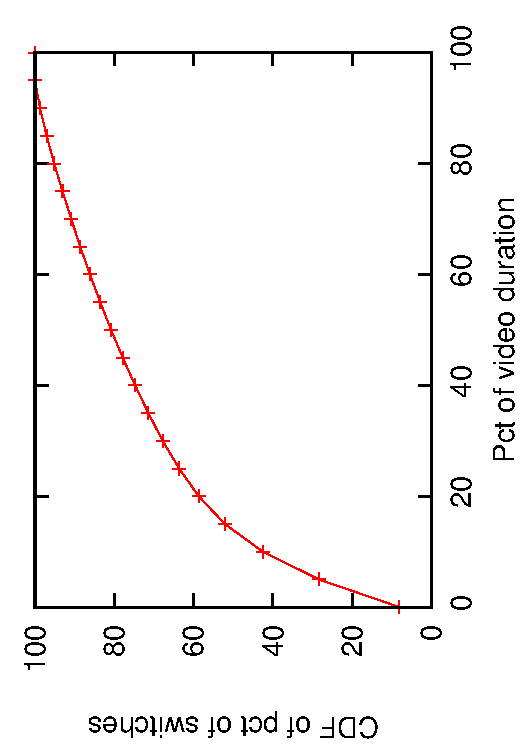
\includegraphics[width=0.3\textwidth] {figures/switch-time-dist.pdf}
\tightcaption{When do adaptive bitrate switches happen? \jc{what's the threshold between long and short form content}}
\label{fig:switch-time-dist}
\end{figure}


\myparatight{Reducing number of  bitrate switch}
We evaluate the switching stability by looking at the number of switches within the first minute of the video play.
We chose one minute because the videos are 5 minutes long and first minute account for 60\% of the switches (see Figure~\ref{fig:switch-time-dist}). 
Since HLS has 10 second video chunks, the maximum number of switches is 6 in this case.
Figure~\ref{subfig:reduce-switch} shows the number of bitrate switches for optimized and random decisions. 
Overall GO can reduce the number of switches by 16\%, and it also increases the number of non-switching-interrupted sessions 
(sessions that experience no switching) by 10\%.
It is possible the reason GO reduces the number of switches is shorter video plays, however, we observed engagement lift
(viewers watch longer because of better quality) at the same time of reduction in number of switches.



\begin{figure}[h!]
\centering
\subfigure[Number of bitrate switches \jc{Xi, revert to last version?}]
{
  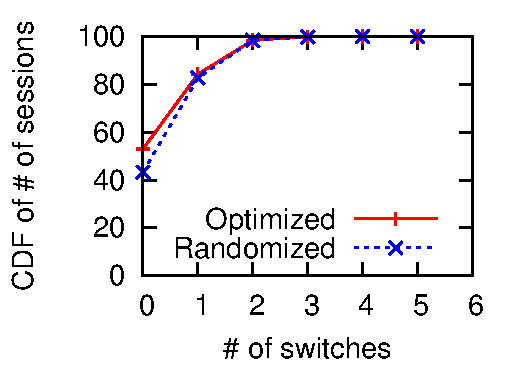
\includegraphics[width=0.24\textwidth] {figures/eval-reduceswitch.pdf}
  \label{subfig:reduce-switch}
}
\hspace{-0.6cm}
\subfigure[Initial vs. dominant bitrate]
{
  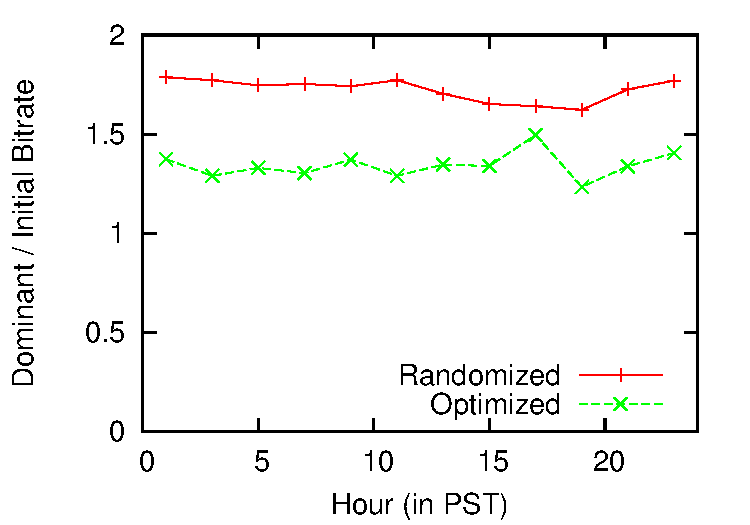
\includegraphics[width=0.24\textwidth] {figures/eval-initvsdom.pdf}
  \label{subfig:initvsdom}
}
\tightcaption{GO improves bitrate adaptation by selecting a better initial bitrate and thus reducing number of bitrate switches.}
\label{fig:bitrate-stability}
\end{figure}


\myparatight{Dominant vs. Initial Bitrate}
Another metric we use to evaluate GO initial bitrate selection is the rate between dominant bitrate and initial bitrate. Dominant bitrate
is the bitrate that the sessions plays for the longest duration, and ideally this number should be 1. Figure~\ref{subfig:initvsdom} shows the ratio of initial bitrate to dominant bitrate. Overall GO is 19\% closer to the dominant bitrate than randomized bitrate selection. 
The figure also shows that for 60\% of the GO-optimized sessions, the initial bitrate selected by GO is almost the same as the dominant bitrate.
%We would like to emphasize again that GO does not make the improvement at the price of engagement, and GO in fact improves engagement.


\tightsubsection{Impact of Policy Constraints}



In summary, our early experience of GO in the real world suggests that it is a promising step towards the global control plane.
